
\chapter{引言:\CTeX 系统的安装和使用}
\label{chap:introduction}

本模板(ustcthesis.cls)是按照教务处的本科论文要求做出的\LaTeX 模板,作者为XPS。\par
本文是使用上述模板生成的示例文档,目的在于帮助使用者熟悉该模板的使用方法,并且方便使用者学位论文的撰写。

\section{系统要求,\CTeX 安装}
本文只针对Windows环境下\CTeX 套装。至于Linux使用者,我觉得你们有能力解决自己的问题。\par
如果电脑上尚未安装\LaTeX 系统,那么到\href{http://www.ctex.org/}{CTeX.org}下载最新完整版\CTeX 套装,并安装之。\par
此模板只支持UTF-8编码。将其他编码的文件转化为UTF-8的方法是: 用记事本打开这些文件, 然后点击文件—另存为—在最下方选择UTF-8 编码。在WinEdt中首次保存时,选择save as...,弹出的窗口中保存类型选择:UTF-8即可。


\section{WinEdit界面介绍和使用}
\CTeX 套装试用WinEdt作为默认编辑器,什么都配置好了,很方便,推荐使用。

打开\CTeX 套装内的WinEdit编辑器,可以看到如图\ref{f:winedit}的界面。
\begin{figure}[ht]
\centering
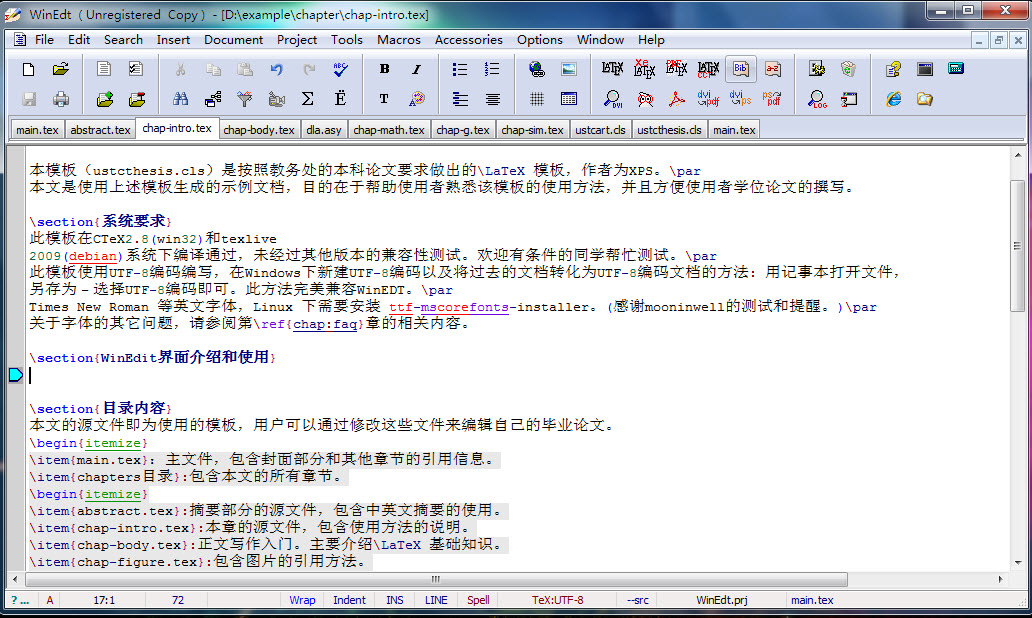
\includegraphics[width=0.8\textwidth]{winedit.jpg}
\caption{WinEdt界面}
\label{f:winedit}
\end{figure}

其中,中部的大块白色背景的区域就是键入文章内容的编辑区。编辑区上方的一条工具栏上有所有当前打开的文件的标签,单击即可跳转到对应文件。标签栏上方是面板,上面有一些很常用的工具按钮,鼠标悬停可以看到按钮名称。下面我们来看其中的几个。在使用本模板时,将会用到这些按钮。
\begin{itemize}
\item 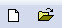
\includegraphics{open.jpg}\\
新建和打开按钮。
\item 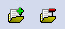
\includegraphics{mainfile.jpg}\\
单击左侧的按钮可设置主文件,单击右侧的取消主文件。
\item 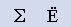
\includegraphics{mathhelp.jpg}\\
单击可以分别打开TeX SYMBOLS GUI(用于输入数学公式)和ASCII字符表。
\item 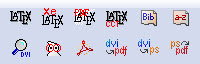
\includegraphics{compile.jpg}\\
编译区,我们需要使用的是上排第二个,第五个和下排第三个,即\XeLaTeX ,BibTeX和 Reader。
\end{itemize}

一般的写作流程是:准备好要写的文字和要插入的图片------在编辑区内输入文字------用各种\LaTeX 命令控制文章格式(第\ref{c:main}章),插入数学公式(第\ref{chap:math}章)、表格(第\ref{chap:tab}章)、图片(第\ref{chap:fig}章)等------编译(\ref{s:compile})------查看结果------修改,再编译------满意的文章。


\section{编译和调试方法}
\label{s:compile}
本模板需要使用\XeLaTeX 编译,切换到main.tex,点击面板上对应的按钮即可。如果你觉得每次都切过来很浪费时间,那么可以换到main.tex,并单击WinEdit工具栏上Set Main File按钮。这样的话以后每次编译都自动从main.tex开始,可以省掉不少麻烦。

如果编译出错,即停在某一位置不动了,且有问号提示符让使用者输入的话,那么按e回车,可以自动跳转到出错位置进行查看。出错的种类五花八门无法一一列举,但是一般都有详细的提示,如果有实在没法修正的可以到BBS TeX板提问。

编译通过之后,可以点工具栏上的Adobe按钮,打开预览。在CTeX2.8套装的WinEdit中,会弹出SumatraPDF,在这个窗口中,看到不合意的地方可以双击回到源文件的相应位置,逆向搜索到原文中的对应位置进行修改,还是比较方便的。\par

\begin{example}{Hello World}\\
将以下内容复制到新文件中,保存为\TeX 文件,编译,然后按Adobe按钮预览结果。
\begin{code}
    \documentclass{article}
    \begin{document}
        Hello world!
    \end{document}
\end{code}
\end{example}


为了得到正确的目录、交叉引用、参考文献等信息,需要编译两到三遍,正确的流程如下:
\begin{enumerate}
\item \XeLaTeX 编译一次。
\item BibTex编译一次。
\item \XeLaTeX 编译两到三次。
\end{enumerate}
在本示例文档中,提供了make.bat,双击之即可完成以上工作。



\section{目录内容}
本文的源文件即为使用的模板,用户可以通过修改这些文件来编辑自己的毕业论文。
\begin{itemize}
\item{main.tex}:主文件,包含封面部分和其他章节的引用信息。
\item{chapters目录}:包含本文的所有章节。
\begin{itemize}
\item{abstract.tex}:摘要部分的源文件,包含中英文摘要的使用。
\item{chap-intro.tex}:本章的源文件,包含使用方法的说明。
\item{chap-body.tex}:正文写作入门。主要介绍\LaTeX 基础知识。
\item{chap-figure.tex}:包含图片的引用方法。
\item{chap-table.tex}:包含表格的示例。
\item{chap-math.tex}:包含数学公式排版的基础知识。
\item{chap-app.tex}:附录。
\item{thanks.tex}包含致谢部分。
\end{itemize}
\item{figures目录}:存放文章内所用的图像文件。
\item{bib/tex.bib}:参考文献信息。
\end{itemize}
需要特别说明的是,这些文件名并不是固定的,你可以新建一个tex文件,例如zhangsan.tex,放在chapters目录下,并且在main.tex中使用
\begin{code}
    \include{chapters/zhangsan.tex}
\end{code}
来引用之。当然你也可以重命名这些文件,只要include中的文件名是存在的,\LaTeX 总能找到这些文件的。

在你写作某一章节的时候,你可能需要随时预览排版效果并debug,这时你可以在其他章节的\verb|\include|命令前加上一个\%,这代表注释掉本行,例如:
\begin{code}
    %%%%%%%%%%%%%%%%%%%%%%%%%%%%%%
    %% 正文部分
    %%%%%%%%%%%%%%%%%%%%%%%%%%%%%%
    \mainmatter
      
\chapter{引言:\CTeX 系统的安装和使用}
\label{chap:introduction}

本模板(ustcthesis.cls)是按照教务处的本科论文要求做出的\LaTeX 模板,作者为XPS。\par
本文是使用上述模板生成的示例文档,目的在于帮助使用者熟悉该模板的使用方法,并且方便使用者学位论文的撰写。

\section{系统要求,\CTeX 安装}
本文只针对Windows环境下\CTeX 套装。至于Linux使用者,我觉得你们有能力解决自己的问题。\par
如果电脑上尚未安装\LaTeX 系统,那么到\href{http://www.ctex.org/}{CTeX.org}下载最新完整版\CTeX 套装,并安装之。\par
此模板只支持UTF-8编码。将其他编码的文件转化为UTF-8的方法是: 用记事本打开这些文件, 然后点击文件—另存为—在最下方选择UTF-8 编码。在WinEdt中首次保存时,选择save as...,弹出的窗口中保存类型选择:UTF-8即可。


\section{WinEdit界面介绍和使用}
\CTeX 套装试用WinEdt作为默认编辑器,什么都配置好了,很方便,推荐使用。

打开\CTeX 套装内的WinEdit编辑器,可以看到如图\ref{f:winedit}的界面。
\begin{figure}[ht]
\centering
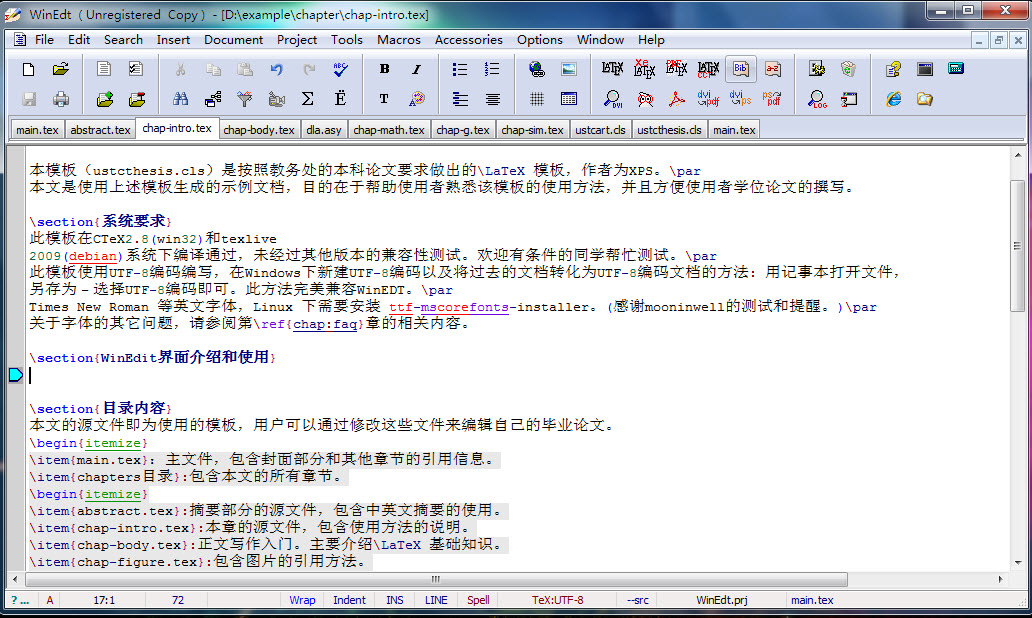
\includegraphics[width=0.8\textwidth]{winedit.jpg}
\caption{WinEdt界面}
\label{f:winedit}
\end{figure}

其中,中部的大块白色背景的区域就是键入文章内容的编辑区。编辑区上方的一条工具栏上有所有当前打开的文件的标签,单击即可跳转到对应文件。标签栏上方是面板,上面有一些很常用的工具按钮,鼠标悬停可以看到按钮名称。下面我们来看其中的几个。在使用本模板时,将会用到这些按钮。
\begin{itemize}
\item 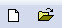
\includegraphics{open.jpg}\\
新建和打开按钮。
\item 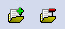
\includegraphics{mainfile.jpg}\\
单击左侧的按钮可设置主文件,单击右侧的取消主文件。
\item 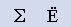
\includegraphics{mathhelp.jpg}\\
单击可以分别打开TeX SYMBOLS GUI(用于输入数学公式)和ASCII字符表。
\item 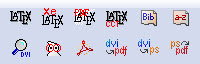
\includegraphics{compile.jpg}\\
编译区,我们需要使用的是上排第二个,第五个和下排第三个,即\XeLaTeX ,BibTeX和 Reader。
\end{itemize}

一般的写作流程是:准备好要写的文字和要插入的图片------在编辑区内输入文字------用各种\LaTeX 命令控制文章格式(第\ref{c:main}章),插入数学公式(第\ref{chap:math}章)、表格(第\ref{chap:tab}章)、图片(第\ref{chap:fig}章)等------编译(\ref{s:compile})------查看结果------修改,再编译------满意的文章。


\section{编译和调试方法}
\label{s:compile}
本模板需要使用\XeLaTeX 编译,切换到main.tex,点击面板上对应的按钮即可。如果你觉得每次都切过来很浪费时间,那么可以换到main.tex,并单击WinEdit工具栏上Set Main File按钮。这样的话以后每次编译都自动从main.tex开始,可以省掉不少麻烦。

如果编译出错,即停在某一位置不动了,且有问号提示符让使用者输入的话,那么按e回车,可以自动跳转到出错位置进行查看。出错的种类五花八门无法一一列举,但是一般都有详细的提示,如果有实在没法修正的可以到BBS TeX板提问。

编译通过之后,可以点工具栏上的Adobe按钮,打开预览。在CTeX2.8套装的WinEdit中,会弹出SumatraPDF,在这个窗口中,看到不合意的地方可以双击回到源文件的相应位置,逆向搜索到原文中的对应位置进行修改,还是比较方便的。\par

\begin{example}{Hello World}\\
将以下内容复制到新文件中,保存为\TeX 文件,编译,然后按Adobe按钮预览结果。
\begin{code}
    \documentclass{article}
    \begin{document}
        Hello world!
    \end{document}
\end{code}
\end{example}


为了得到正确的目录、交叉引用、参考文献等信息,需要编译两到三遍,正确的流程如下:
\begin{enumerate}
\item \XeLaTeX 编译一次。
\item BibTex编译一次。
\item \XeLaTeX 编译两到三次。
\end{enumerate}
在本示例文档中,提供了make.bat,双击之即可完成以上工作。



\section{目录内容}
本文的源文件即为使用的模板,用户可以通过修改这些文件来编辑自己的毕业论文。
\begin{itemize}
\item{main.tex}:主文件,包含封面部分和其他章节的引用信息。
\item{chapters目录}:包含本文的所有章节。
\begin{itemize}
\item{abstract.tex}:摘要部分的源文件,包含中英文摘要的使用。
\item{chap-intro.tex}:本章的源文件,包含使用方法的说明。
\item{chap-body.tex}:正文写作入门。主要介绍\LaTeX 基础知识。
\item{chap-figure.tex}:包含图片的引用方法。
\item{chap-table.tex}:包含表格的示例。
\item{chap-math.tex}:包含数学公式排版的基础知识。
\item{chap-app.tex}:附录。
\item{thanks.tex}包含致谢部分。
\end{itemize}
\item{figures目录}:存放文章内所用的图像文件。
\item{bib/tex.bib}:参考文献信息。
\end{itemize}
需要特别说明的是,这些文件名并不是固定的,你可以新建一个tex文件,例如zhangsan.tex,放在chapters目录下,并且在main.tex中使用
\begin{code}
    \include{chapters/zhangsan.tex}
\end{code}
来引用之。当然你也可以重命名这些文件,只要include中的文件名是存在的,\LaTeX 总能找到这些文件的。

在你写作某一章节的时候,你可能需要随时预览排版效果并debug,这时你可以在其他章节的\verb|\include|命令前加上一个\%,这代表注释掉本行,例如:
\begin{code}
    %%%%%%%%%%%%%%%%%%%%%%%%%%%%%%
    %% 正文部分
    %%%%%%%%%%%%%%%%%%%%%%%%%%%%%%
    \mainmatter
      
\chapter{引言:\CTeX 系统的安装和使用}
\label{chap:introduction}

本模板(ustcthesis.cls)是按照教务处的本科论文要求做出的\LaTeX 模板,作者为XPS。\par
本文是使用上述模板生成的示例文档,目的在于帮助使用者熟悉该模板的使用方法,并且方便使用者学位论文的撰写。

\section{系统要求,\CTeX 安装}
本文只针对Windows环境下\CTeX 套装。至于Linux使用者,我觉得你们有能力解决自己的问题。\par
如果电脑上尚未安装\LaTeX 系统,那么到\href{http://www.ctex.org/}{CTeX.org}下载最新完整版\CTeX 套装,并安装之。\par
此模板只支持UTF-8编码。将其他编码的文件转化为UTF-8的方法是: 用记事本打开这些文件, 然后点击文件—另存为—在最下方选择UTF-8 编码。在WinEdt中首次保存时,选择save as...,弹出的窗口中保存类型选择:UTF-8即可。


\section{WinEdit界面介绍和使用}
\CTeX 套装试用WinEdt作为默认编辑器,什么都配置好了,很方便,推荐使用。

打开\CTeX 套装内的WinEdit编辑器,可以看到如图\ref{f:winedit}的界面。
\begin{figure}[ht]
\centering
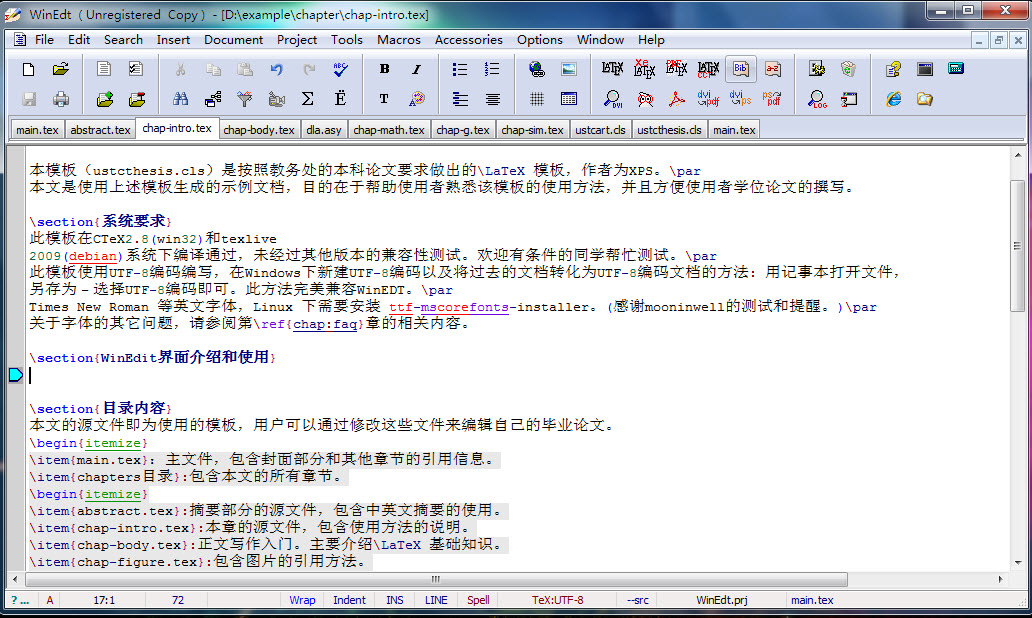
\includegraphics[width=0.8\textwidth]{winedit.jpg}
\caption{WinEdt界面}
\label{f:winedit}
\end{figure}

其中,中部的大块白色背景的区域就是键入文章内容的编辑区。编辑区上方的一条工具栏上有所有当前打开的文件的标签,单击即可跳转到对应文件。标签栏上方是面板,上面有一些很常用的工具按钮,鼠标悬停可以看到按钮名称。下面我们来看其中的几个。在使用本模板时,将会用到这些按钮。
\begin{itemize}
\item 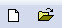
\includegraphics{open.jpg}\\
新建和打开按钮。
\item 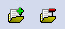
\includegraphics{mainfile.jpg}\\
单击左侧的按钮可设置主文件,单击右侧的取消主文件。
\item 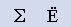
\includegraphics{mathhelp.jpg}\\
单击可以分别打开TeX SYMBOLS GUI(用于输入数学公式)和ASCII字符表。
\item 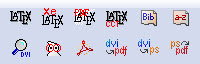
\includegraphics{compile.jpg}\\
编译区,我们需要使用的是上排第二个,第五个和下排第三个,即\XeLaTeX ,BibTeX和 Reader。
\end{itemize}

一般的写作流程是:准备好要写的文字和要插入的图片------在编辑区内输入文字------用各种\LaTeX 命令控制文章格式(第\ref{c:main}章),插入数学公式(第\ref{chap:math}章)、表格(第\ref{chap:tab}章)、图片(第\ref{chap:fig}章)等------编译(\ref{s:compile})------查看结果------修改,再编译------满意的文章。


\section{编译和调试方法}
\label{s:compile}
本模板需要使用\XeLaTeX 编译,切换到main.tex,点击面板上对应的按钮即可。如果你觉得每次都切过来很浪费时间,那么可以换到main.tex,并单击WinEdit工具栏上Set Main File按钮。这样的话以后每次编译都自动从main.tex开始,可以省掉不少麻烦。

如果编译出错,即停在某一位置不动了,且有问号提示符让使用者输入的话,那么按e回车,可以自动跳转到出错位置进行查看。出错的种类五花八门无法一一列举,但是一般都有详细的提示,如果有实在没法修正的可以到BBS TeX板提问。

编译通过之后,可以点工具栏上的Adobe按钮,打开预览。在CTeX2.8套装的WinEdit中,会弹出SumatraPDF,在这个窗口中,看到不合意的地方可以双击回到源文件的相应位置,逆向搜索到原文中的对应位置进行修改,还是比较方便的。\par

\begin{example}{Hello World}\\
将以下内容复制到新文件中,保存为\TeX 文件,编译,然后按Adobe按钮预览结果。
\begin{code}
    \documentclass{article}
    \begin{document}
        Hello world!
    \end{document}
\end{code}
\end{example}


为了得到正确的目录、交叉引用、参考文献等信息,需要编译两到三遍,正确的流程如下:
\begin{enumerate}
\item \XeLaTeX 编译一次。
\item BibTex编译一次。
\item \XeLaTeX 编译两到三次。
\end{enumerate}
在本示例文档中,提供了make.bat,双击之即可完成以上工作。



\section{目录内容}
本文的源文件即为使用的模板,用户可以通过修改这些文件来编辑自己的毕业论文。
\begin{itemize}
\item{main.tex}:主文件,包含封面部分和其他章节的引用信息。
\item{chapters目录}:包含本文的所有章节。
\begin{itemize}
\item{abstract.tex}:摘要部分的源文件,包含中英文摘要的使用。
\item{chap-intro.tex}:本章的源文件,包含使用方法的说明。
\item{chap-body.tex}:正文写作入门。主要介绍\LaTeX 基础知识。
\item{chap-figure.tex}:包含图片的引用方法。
\item{chap-table.tex}:包含表格的示例。
\item{chap-math.tex}:包含数学公式排版的基础知识。
\item{chap-app.tex}:附录。
\item{thanks.tex}包含致谢部分。
\end{itemize}
\item{figures目录}:存放文章内所用的图像文件。
\item{bib/tex.bib}:参考文献信息。
\end{itemize}
需要特别说明的是,这些文件名并不是固定的,你可以新建一个tex文件,例如zhangsan.tex,放在chapters目录下,并且在main.tex中使用
\begin{code}
    \include{chapters/zhangsan.tex}
\end{code}
来引用之。当然你也可以重命名这些文件,只要include中的文件名是存在的,\LaTeX 总能找到这些文件的。

在你写作某一章节的时候,你可能需要随时预览排版效果并debug,这时你可以在其他章节的\verb|\include|命令前加上一个\%,这代表注释掉本行,例如:
\begin{code}
    %%%%%%%%%%%%%%%%%%%%%%%%%%%%%%
    %% 正文部分
    %%%%%%%%%%%%%%%%%%%%%%%%%%%%%%
    \mainmatter
      
\chapter{引言:\CTeX 系统的安装和使用}
\label{chap:introduction}

本模板(ustcthesis.cls)是按照教务处的本科论文要求做出的\LaTeX 模板,作者为XPS。\par
本文是使用上述模板生成的示例文档,目的在于帮助使用者熟悉该模板的使用方法,并且方便使用者学位论文的撰写。

\section{系统要求,\CTeX 安装}
本文只针对Windows环境下\CTeX 套装。至于Linux使用者,我觉得你们有能力解决自己的问题。\par
如果电脑上尚未安装\LaTeX 系统,那么到\href{http://www.ctex.org/}{CTeX.org}下载最新完整版\CTeX 套装,并安装之。\par
此模板只支持UTF-8编码。将其他编码的文件转化为UTF-8的方法是: 用记事本打开这些文件, 然后点击文件—另存为—在最下方选择UTF-8 编码。在WinEdt中首次保存时,选择save as...,弹出的窗口中保存类型选择:UTF-8即可。


\section{WinEdit界面介绍和使用}
\CTeX 套装试用WinEdt作为默认编辑器,什么都配置好了,很方便,推荐使用。

打开\CTeX 套装内的WinEdit编辑器,可以看到如图\ref{f:winedit}的界面。
\begin{figure}[ht]
\centering
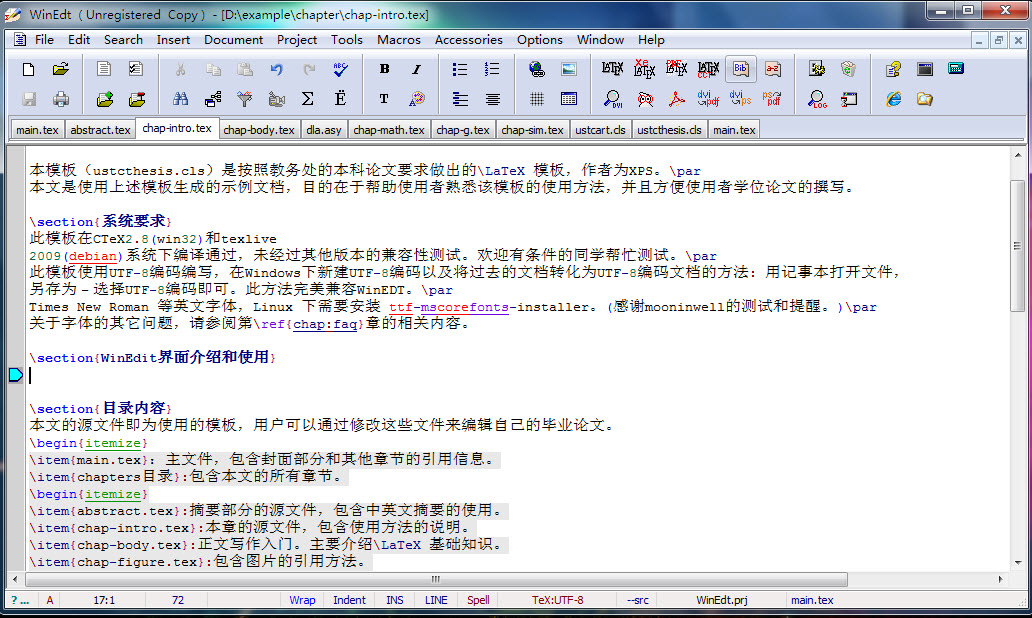
\includegraphics[width=0.8\textwidth]{winedit.jpg}
\caption{WinEdt界面}
\label{f:winedit}
\end{figure}

其中,中部的大块白色背景的区域就是键入文章内容的编辑区。编辑区上方的一条工具栏上有所有当前打开的文件的标签,单击即可跳转到对应文件。标签栏上方是面板,上面有一些很常用的工具按钮,鼠标悬停可以看到按钮名称。下面我们来看其中的几个。在使用本模板时,将会用到这些按钮。
\begin{itemize}
\item 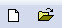
\includegraphics{open.jpg}\\
新建和打开按钮。
\item 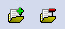
\includegraphics{mainfile.jpg}\\
单击左侧的按钮可设置主文件,单击右侧的取消主文件。
\item 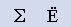
\includegraphics{mathhelp.jpg}\\
单击可以分别打开TeX SYMBOLS GUI(用于输入数学公式)和ASCII字符表。
\item 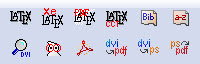
\includegraphics{compile.jpg}\\
编译区,我们需要使用的是上排第二个,第五个和下排第三个,即\XeLaTeX ,BibTeX和 Reader。
\end{itemize}

一般的写作流程是:准备好要写的文字和要插入的图片------在编辑区内输入文字------用各种\LaTeX 命令控制文章格式(第\ref{c:main}章),插入数学公式(第\ref{chap:math}章)、表格(第\ref{chap:tab}章)、图片(第\ref{chap:fig}章)等------编译(\ref{s:compile})------查看结果------修改,再编译------满意的文章。


\section{编译和调试方法}
\label{s:compile}
本模板需要使用\XeLaTeX 编译,切换到main.tex,点击面板上对应的按钮即可。如果你觉得每次都切过来很浪费时间,那么可以换到main.tex,并单击WinEdit工具栏上Set Main File按钮。这样的话以后每次编译都自动从main.tex开始,可以省掉不少麻烦。

如果编译出错,即停在某一位置不动了,且有问号提示符让使用者输入的话,那么按e回车,可以自动跳转到出错位置进行查看。出错的种类五花八门无法一一列举,但是一般都有详细的提示,如果有实在没法修正的可以到BBS TeX板提问。

编译通过之后,可以点工具栏上的Adobe按钮,打开预览。在CTeX2.8套装的WinEdit中,会弹出SumatraPDF,在这个窗口中,看到不合意的地方可以双击回到源文件的相应位置,逆向搜索到原文中的对应位置进行修改,还是比较方便的。\par

\begin{example}{Hello World}\\
将以下内容复制到新文件中,保存为\TeX 文件,编译,然后按Adobe按钮预览结果。
\begin{code}
    \documentclass{article}
    \begin{document}
        Hello world!
    \end{document}
\end{code}
\end{example}


为了得到正确的目录、交叉引用、参考文献等信息,需要编译两到三遍,正确的流程如下:
\begin{enumerate}
\item \XeLaTeX 编译一次。
\item BibTex编译一次。
\item \XeLaTeX 编译两到三次。
\end{enumerate}
在本示例文档中,提供了make.bat,双击之即可完成以上工作。



\section{目录内容}
本文的源文件即为使用的模板,用户可以通过修改这些文件来编辑自己的毕业论文。
\begin{itemize}
\item{main.tex}:主文件,包含封面部分和其他章节的引用信息。
\item{chapters目录}:包含本文的所有章节。
\begin{itemize}
\item{abstract.tex}:摘要部分的源文件,包含中英文摘要的使用。
\item{chap-intro.tex}:本章的源文件,包含使用方法的说明。
\item{chap-body.tex}:正文写作入门。主要介绍\LaTeX 基础知识。
\item{chap-figure.tex}:包含图片的引用方法。
\item{chap-table.tex}:包含表格的示例。
\item{chap-math.tex}:包含数学公式排版的基础知识。
\item{chap-app.tex}:附录。
\item{thanks.tex}包含致谢部分。
\end{itemize}
\item{figures目录}:存放文章内所用的图像文件。
\item{bib/tex.bib}:参考文献信息。
\end{itemize}
需要特别说明的是,这些文件名并不是固定的,你可以新建一个tex文件,例如zhangsan.tex,放在chapters目录下,并且在main.tex中使用
\begin{code}
    \include{chapters/zhangsan.tex}
\end{code}
来引用之。当然你也可以重命名这些文件,只要include中的文件名是存在的,\LaTeX 总能找到这些文件的。

在你写作某一章节的时候,你可能需要随时预览排版效果并debug,这时你可以在其他章节的\verb|\include|命令前加上一个\%,这代表注释掉本行,例如:
\begin{code}
    %%%%%%%%%%%%%%%%%%%%%%%%%%%%%%
    %% 正文部分
    %%%%%%%%%%%%%%%%%%%%%%%%%%%%%%
    \mainmatter
      \include{chapter/chap-intro}
    %  \include{chapter/chap-figure}
    %  \include{chapter/chap-table}
    %  \include{chapter/chap-math}
    %  \include{chapter/chap-faq}
\end{code}
那么,编译的时候就只编译未加\%的一章,在这个例子中,即本章。

理论上,并不一定要把每章放在不同的文件中,但是这种分章节写作、编译的方法有利于提高效率,大大减少debug过程中的编译时间,同时减小风险。 
    %  
\chapter{图形}
\label{chap:fig}


\section{浮动图形}

\XeLaTeX 支持jpg和eps格式的图片。我们所用的编译方法支持jpg和eps等格式的图片。如果你已经有一篇word文档,
想把其中的图全部导出,那么可以将它另存为html文件,这时会在同目录下找到一个文件夹,里面是所有用到的图片。

将插图放在figures文件夹中,想要引用的地方使用类似这样的命令插入图形文件:
\begin{code}
\begin{figure}[!ht]
 \centering
 
\includegraphics[width=0.2\textwidth]{ustc_logo_new.eps}
 \caption{中国科学技术大学校徽(在页面中间)}
 \label{fig:ustc1}
\end{figure}
\end{code}
结果如下:
\begin{figure}[!ht]
 \centering
 
\includegraphics[width=0.2\textwidth]{ustc_logo_new.eps}
 \caption{中国科学技术大学校徽(在页面中间)}
 \label{fig:ustc1}
\end{figure}

在上面这段命令中,可选参数[!ht]代表插图的位置。其中!让\LaTeX{}忽略审美标准,试图用最严格的标准来放置浮动图形;h(ere)代表有限放在此处;t(op)代表如果此处放不下,那么放在下一页页首。

width=0.2\textbackslash{}textwidth代表图形的宽度是文字宽度的0.2倍,你也可以使用其他长度单位,如12cm,4.5in等等。

caption命令的参数代表图的名称,或者说注解。label的参数用于交叉引用,见下节。


\section{交叉引用}
通过使用交叉引用功能,我们可以定位那些\LaTeX{}自动编号的内容,比如浮动图形、表格、章节等等。其中,label和ref的参数是引用的名字,可以随意,但须保持一致。
\begin{figure}[ht]
\centering
\fbox{\begin{minipage}[h]{0.4\textwidth}
引用图\ref{fig:ustc1}\\
引用第\ref{chap:introduction}章
\end{minipage}}
\hspace{0.1\textwidth}
\begin{minipage}[h]{0.4\textwidth}
\centering
\begin{code}
引用图\ref{fig:ustc1}\\
引用第\ref{chap:introduction}章
\end{code}
\end{minipage}
\caption{交叉引用示例}
\end{figure}


\section{并列的子图}
使用subfigure命令,一个例子:
\begin{figure}[!hbt]
\centering
\subfigure[sf 1]{

\includegraphics[width=0.2\textwidth]{ustc_logo_new.eps}\label{f:1}}
\subfigure[sf 2]{

\includegraphics[width=0.2\textwidth]{ustc_logo_new.eps}\label{f:2}}
\subfigure[sf 3]{

\includegraphics[width=0.2\textwidth]{ustc_logo_new.eps}\label{f:3}}
\subfigure[sf 4]{

\includegraphics[width=0.2\textwidth]{ustc_logo_new.eps}\label{f:4}}
\caption{\label{f:s}subfigure使用示例。}
\end{figure}
\begin{code}
\begin{figure}[!hbt]
\centering
\subfigure[sf 1]{

\includegraphics[width=0.2\textwidth]{ustc_logo_new.eps}\label{f:1}}
\subfigure[sf 2]{

\includegraphics[width=0.2\textwidth]{ustc_logo_new.eps}\label{f:2}}
\subfigure[sf 3]{

\includegraphics[width=0.2\textwidth]{ustc_logo_new.eps}\label{f:3}}
\subfigure[sf 4]{

\includegraphics[width=0.2\textwidth]{ustc_logo_new.eps}\label{f:4}}
\caption{\label{f:s}subfigure使用示例。}
\end{figure}
\end{code}

分两行放:
\begin{figure}[!hbt]
\centering
\subfigure[sf 1]{

\includegraphics[width=0.2\textwidth]{ustc_logo_new.eps}\label{f:1}}
\subfigure[sf 2]{

\includegraphics[width=0.2\textwidth]{ustc_logo_new.eps}\label{f:2}}\\
\subfigure[sf 3]{

\includegraphics[width=0.2\textwidth]{ustc_logo_new.eps}\label{f:3}}
\subfigure[sf 4]{

\includegraphics[width=0.2\textwidth]{ustc_logo_new.eps}\label{f:4}}
\caption{\label{f:s}subfigure使用示例。}
\end{figure}
\begin{code}
\begin{figure}[!hbt]
\centering
\subfigure[f 1]{

\includegraphics[width=0.2\textwidth]{ustc_logo_new.eps}\label{f:1}}
\subfigure[f 2]{

\includegraphics[width=0.2\textwidth]{ustc_logo_new.eps}\label{f:2}}\\
\subfigure[f 3]{

\includegraphics[width=0.2\textwidth]{ustc_logo_new.eps}\label{f:3}}
\subfigure[f 4]{

\includegraphics[width=0.2\textwidth]{ustc_logo_new.eps}\label{f:4}}
\caption{\label{f:l}分行的字图使用示例。}
\end{figure}
\end{code}
    %  
\chapter{表格}
\label{chap:tab}
标准三线表:
\begin{table}[!ht]
\label{tab:table3}
\caption{三线表格示例}
\centering
\begin{tabular}{c c c c}
\whline 一列 & 两列 & 三列 & 四列  \\\hline
1 & 2 &3 &4 \\2 & 3 &4 &5 \\3 & 4 &5 &6 \\
\whline
\end{tabular}
\end{table}
\begin{code}
    \begin{table}[!ht]
    \label{tab:table3}
    \caption{三线表格示例}
    \centering
    \begin{tabular}{c c c c}
        \whline 一列 & 两列 & 三列 & 四列  \\\whline
        1 & 2 &3 &4 \\2 & 3 &4 &5 \\3 & 4 &5 &6 \\
        \whline
    \end{tabular}
    \end{table}
\end{code}

与figure一样,table环境也是浮动体,常用!ht来表明位置。caption、label的意义都与figure环境相同。

而画表格的tabular环境则与array环境几乎相同,只是在每行之间可以用\textbackslash{}hline和\textbackslash{}hline这些命令来画横线。c代表一个居中对齐的列,l代表靠左对齐,r代表靠右对齐。
有竖线的例子:
\begin{table}[!ht]
\label{tab:table2}
\caption{表格示例2}
\centering
\begin{tabular}{ Ic|c|c|cI}
\whline 一列 & 两列 & 三列 & 四列  \\\hline
1 & 2 &3 &4 \\\hline 2 & 3 &4 &5 \\\hline3 & 4 &5 &6 \\
\whline
\end{tabular}
\end{table}
\begin{code}
    \begin{table}[!ht]
    \label{tab:table2}
    \caption{表格示例2}
    \centering
    \begin{tabular}{ Ic|c|c|cI}
        \whline 一列 & 两列 & 三列 & 四列  \\\hline
        1 & 2 &3 &4 \\\hline 2 & 3 &4 &5 \\\hline3 & 4 &5 &6 \\
        \whline
    \end{tabular}
    \end{table}
\end{code}

即竖线是|,粗竖线是大写字母I,横线是\textbackslash hline,粗横线是\textbackslash whline。

    %  
\chapter{数学公式}
\label{chap:math}
数学公式需在数学环境中排版。数学环境一般分\textit{正文公式}和\textit{显示公式}。正文公式用\verb|$...$|表示,而显示公式则用equation,align等数学环境。简单的几个例子:
\begin{figure}[ht]
\centering
\fbox{\begin{minipage}[h]{0.4\textwidth}
这是一个显示公式:
    \begin{equation}
    x+y=z
    \end{equation}
谢谢。
\end{minipage}}
\hspace{0.1\textwidth}
\begin{minipage}[h]{0.4\textwidth}
\centering
\begin{code}
这是一个显示公式:
\begin{equation}
x+y=z
\end{equation}
谢谢。
\end{code}
\end{minipage}
\caption{显示公式}
\end{figure}
\begin{figure}[h]
\centering
\fbox{\begin{minipage}[c]{0.4\textwidth}
大家好,$e^{\pi i}+1=0$是我最喜欢的方程。
\end{minipage}}
\hspace{0.1\textwidth}
\begin{minipage}[h]{0.4\textwidth}
\centering
\begin{code}
大家好,$e^{\pi i}+1=0$是我最喜欢的方程。
\end{code}
\end{minipage}
\caption{正文公式}
\end{figure}

常用的显示公式环境有:
\begin{itemize}
\item{equation}:最常用的公式环境。
\item{displaymath}:与equation的差别在于不会被自动编号。\\
\verb|\begin{displaymath}...\end{displaymath}|可以用\verb|\[...\]|来代替。
\item{align}:适用于排版多个需要对齐的公式。
\end{itemize}


\section{数学公式排版基础}
上下标、希腊字母、加减乘除等常用符号:
\begin{center}
\begin{tabular}{ccll}
\whline
& 命令 & 例子 & 代码\\
\hline
上标 & \^{} & $x^2$ & \verb|$x^2$|\\
下标 & \_{} & $x_2$ & \verb|$x_2$|\\
希腊字母 & 对应的英文 & $\pi,\rho,\sigma,...$ &\verb|$\pi,\rho,\sigma,...$|\\
点乘 & \verb|\cdot| & $x\cdot y$ & \verb|$x\cdot y$|\\
叉乘 & \verb|\times| & $x\times y$ & \verb|$x\times y$|\\
分数 & \verb|\frac{}{}| & $\frac{abc}{def}$ &\verb|$\frac{abc}{def}$|\\
根号 & \verb|\sqrt[n]{}|  & $\sqrt{x},\sqrt[3]{y}$ &\verb|$\sqrt{x},\sqrt[3]{y}$|\\
积分 &\verb|\int|  & $\int,\iint,\iiint$ & \verb|$\int,\iint,\iiint$|\\
\whline
\end{tabular}
\end{center}
表中,\$代表数学环境。在equation等环境中排版时,不再需要使用\$符号。

更多的符号,请点击WinEdt面板上的$\Sigma$符号(TeX Symbols GUI),在弹出的面板中查找。

当控制符作用于多个字符时,需要用大括号将这些字符都括起来,如
\begin{center}
\begin{tabular}{c c}
\whline
例子 & 代码\\
\hline
$e^{\pi i}+1=0$ & \verb|e^{\pi i}+1=0|\\
$x_{12}^{3}$ & \verb|x_{12}^{3}|\\
${x_{12}}^{3}$ & \verb|{x_{12}}^{3}|\\
\whline
\end{tabular}
\end{center}

\section{控制字体}
本科学位论文对于公式内字体的使用有严格的规定。一般变量用白斜体,常量和特殊函数等用白正体,矢量用黑斜体,张量用黑正体。改变字体的命令如下表:
\begin{center}
\begin{tabular}{c c l l}
\whline
& 字体 & 例子 & 代码\\
\hline
一般变量 & 白斜体 & $x$ & \verb|$x$|\\
常量  & 白正体 & $\mathrm{c}$  & \verb|$\mathrm{c}$|\\
矢量  & 黑斜体 & $\bm{B}$ & \verb|$\bm{B}$|\\
张量  & 黑正体 & $\mathbf{H}$ & \verb|$\mathbf{H}$|\\
\whline
\end{tabular}
\end{center}
表中,\$代表数学环境。在equation等环境中排版时,不再需要使用\$符号。

\section{括号}
中括号、小括号和竖线可以用键盘上对应的键来输入。大括号是\LaTeX{}中的控制符,必须用\verb|\{...\}|来输入。态函数所用的尖括号是\verb|\langle|和\verb|\rangle|。一个句点代表一个不显示的括号。

使用\verb|\left|和\verb|\right|可以自动控制括号的大小。使用时,将所需要用的括号紧跟在\verb|\left|或\verb|\right|后面就好。例如:
\begin{figure}[ht]
\centering
\fbox{\begin{minipage}[h]{0.8\textwidth}
    \[
    \left[\frac{\left(\frac{abc}{def}+ghi\right)\cdot jkl}{mno}+pqr\right]\times st=0
    \]
\end{minipage}}\\
\vskip10pt
\begin{minipage}[h]{0.8\textwidth}
\centering
\begin{code}
\[
\left[\frac{\left(\frac{abc}{def}+ghi\right)\cdot jkl}{mno}+pqr\right]
\times st=0
\]
\end{code}
\end{minipage}
\caption{括号。\textbackslash[和\textbackslash]代表displaymath环境,下同。}
\end{figure}



使用括号时,不一定要用相同的括号来匹配。甚至可以用\verb|\left.|这样不被显示括号来匹配正常括号,以达到排版目的。如
\begin{figure}[h]
\centering
\fbox{\begin{minipage}[h]{0.4\textwidth}
\[\left|\psi\right\rangle\]
\end{minipage}}
\hspace{0.1\textwidth}
\begin{minipage}[h]{0.4\textwidth}
\centering
\begin{code}
\[\left|\psi\right\rangle\]
\end{code}
\end{minipage}\\
\vskip10pt
\fbox{\begin{minipage}[h]{0.4\textwidth}
\[\left\{
\begin{array}{c}
a\\b\\c
\end{array}
\right.\]
\end{minipage}}
\hspace{0.1\textwidth}
\begin{minipage}[h]{0.4\textwidth}
\centering
\begin{code}
\[\left\{\begin{array}{c}
a\\b\\c
\end{array}\right.\]
\end{code}
\end{minipage}
\caption{不同括号的匹配}
\end{figure}

\section{矩阵}
输入矩阵一般使用array环境。

矩阵中使用\verb|&|来分位,\verb|\\|来分行。array环境的参数指定了列的数量和每列的对齐方式。c代表一个居中对齐的列,l是靠左对齐,r则是靠右对齐。图\ref{f:matrix}是一个简单的例子。
\begin{figure}[h]
\centering
\fbox{\begin{minipage}[h]{0.4\textwidth}
\[\left[
\begin{array}{c c c}
C_{Xx} & C_{Yx} & C_{Zx}\\
C_{Xy} & C_{Yy} & C_{Zy}\\
C_{Xz} & C_{Yz} & C_{Zz}
\end{array}
\right]\]
\end{minipage}}
\hspace{0.1\textwidth}
\begin{minipage}[h]{0.4\textwidth}
\centering
\begin{code}
\[\left[\begin{array}{c c c}
C_{Xx} & C_{Yx} & C_{Zx}\\
C_{Xy} & C_{Yy} & C_{Zy}\\
C_{Xz} & C_{Yz} & C_{Zz}
\end{array}\right]\]
\end{code}
\end{minipage}
\caption{矩阵}
\label{f:matrix}
\end{figure}

array环境可以自嵌套,达到输入复杂矩阵的目的。

\section{对齐的多行公式}
align环境提供了书写多行公式,并指定其在某一位置对齐的功能,使用\&来代表对齐点。如图\ref{f:align}。其中,\verb|\notag| 表示不对这一行公式进行编号。
\begin{figure}[h]
\centering
\fbox{\begin{minipage}[b]{0.8\textwidth}
\begin{align}
a_0&=(A_1+A_2+A_3)/3\textrm{g}_e\beta_e\\
b_0&=[A_1-(A_2+A_3)/2]/3\textrm{g}_e\beta_e\notag\\
c_0&=(|A_2|-|A_3|)/2\textrm{g}_e\beta_e
\end{align}
\end{minipage}}\\
\begin{minipage}[b]{0.8\textwidth}
\centering
\begin{code}
\begin{align}
a_0&=(A_1+A_2+A_3)/3\textrm{g}_e\beta_e\\
b_0&=[A_1-(A_2+A_3)/2]/3\textrm{g}_e\beta_e\notag\\
c_0&=(|A_2|-|A_3|)/2\textrm{g}_e\beta_e
\end{align}
\end{code}
\end{minipage}
\caption{多行公式}
\label{f:align}
\end{figure}

\section{定理,证明,和其他环境}
ustcthesis中提供了定理,证明等一些其他环境。环境和名称如下表:
\begin{center}
\begin{tabular}{l l @\qquad l l}
\whline
环境名 & 中文名 &环境名 & 中文名\\
\hline
theorem & 定理&
lemma&引理\\
example&例&
algorithm&算法\\
definition&定义&
axiom&公理\\
property&性质&
proposition&命题\\
corollary&推论&
remark&注解\\
condition&条件&
conclusion&结论\\
assumption&假设&
prove&证明\\
\whline
\end{tabular}
\end{center}

    %  \def\Q{\noindent Question:~~}
\def\A{\newline Answer:~~}
\chapter{FAQ}
\label{chap:contact}

这里是我们已经收到的一些常见问题以及一些一般的Debug技巧. 对于更多的信息或者关于本模板和文档的任何疑问,请移步\href{http://bbs.ustc.edu.cn/cgi/bbsdoc?board=TeX}{瀚海星云\TeX{}讨论区}。

\Q 从哪里下载\CTeX{}套装? 应该下载哪一个\CTeX{}套装?
\A 在\href{http://www.ctex.org}{\CTeX{}官方网站}可以下载, 进入网站后点击网页右边的``项目''栏目中``最新稳定版'', 即可进入下载链接. 对于有良好网络链接的同学, 我们强烈建议下载较大的那个完全版, 实在是网络速度不佳的同学可以下载精简版的, 但是编译的时候会经常实时下载某些宏包, 很麻烦, 因此不推荐.

\Q 我自己新建了一个文件并且写了一段文字, 为什么编译出来的中文是乱码呢? 但是用模板里面的文件编译正常.
\A 请仔细确认你新建的文件是不是UTF-8编码! 如果不是, 请按文章前述方法转换成UTF-8编码.

\Q 我编译总是报错, 按e定位总是定位到主文件?
\A 这种问题比较复杂, 可能是你的某个正文中的命令与模板冲突, 或者有时与宏包冲突也会出现这种情况. 这时我们只能手动定位错误, 具体方式如下: 首先确定问题在哪一章? 方法是一章一章的编译, 然后确定问题在哪一节, 方法是只编译问题章节, 然后一节一节的编译. 最后确定问题在哪一行. 一般对于新手而言, 容易在数学公式中出问题, 所以, 请优先检查数学公式. 这样通过逐级定位, 我们就可以精确的获知错误的位置, 然后仔细检查, 就可以得到错误的原因, 即使你无法理解错误, 也可以对症求医, 在\TeX{}版求问.

\Q 编译错误时, DOS窗口里报了一大堆英文, 如何看懂啊?
\A 前面的都是编译信息不用理睬, 后面的是错误信息要仔细看, 比如这一段
\begin{code}
  ! Undefined control sequence.
l.16 \adga
           agasgarga
?
\end{code}
这一段有4行, 最后一行是问你如何处理, 我们在这里输入我们的处理方案. 现在看前三行. 第一行由一个感叹号开头, 这里是错误原因, 说明我用了一个没有定义的命令.
第二行是\verb|l.16|开头, 说明第16行出问题了, 然后这里有一个断行, 这个断行表示错误的精确位置, 这里, 由于没有\verb|\adga|这个命令, 自然就会报错.
后面的第三行是辅助文字, 表示错误后面的一些代码, 这样可以方便我们精确定位, 这种显示方式在大段的数学公式出错时尤其方便. 至于第4行, 前述办法是: 一般按E, 回车, 方便的在代码中回溯到我们需要的行. 在这里我们再介绍一个命令: h---回车. h的意思是help, 这样, \TeX{}的编译器会使用尽可能你熟悉的语言告诉你具体为什么错了. 有的时候这是很有帮助的, 而有的时候你却完全不知道他在说什么. 这是很正常的, 因为电脑的长处在于执行命令, 而不是主动读懂你的想法.(Knuth in TeXbook)

\Q 一个诡异的错误:
\A 也许你已经学习了一些公式的编写, 那么, 请看下面一段代码:
\begin{code}
\begin{eqnarray}
  [X_1, X_2] &=& 0\\
  [X_3, X_4] &=& Q_{\pm}
\end{eqnarray}
\end{code}
你肯定觉得这是个很简单的括号问题, 但是实际上这是无法编译的! 解决方案是在第一行公式后面加上\verb|\relax|, 原因很巧妙, 换行符\verb|\\|后面的中括号代表该命令的可选参数, 表示空多少尺寸, 在上述公式中, 第二行的公式恰好是以\verb|[|开头, 自然无法编译过去. 这在TeXbook中叫做``weird mistakes''. 其实, 我们有很多可能遇到各种诡异的问题, 有时这种问题的思路是超越我们的想法的, 因此, 希望大家可以多多发问, 善于在网络上与同学们讨论问题, 这样才能有助于问题的解决.



\end{code}
那么,编译的时候就只编译未加\%的一章,在这个例子中,即本章。

理论上,并不一定要把每章放在不同的文件中,但是这种分章节写作、编译的方法有利于提高效率,大大减少debug过程中的编译时间,同时减小风险。 
    %  
\chapter{图形}
\label{chap:fig}


\section{浮动图形}

\XeLaTeX 支持jpg和eps格式的图片。我们所用的编译方法支持jpg和eps等格式的图片。如果你已经有一篇word文档,
想把其中的图全部导出,那么可以将它另存为html文件,这时会在同目录下找到一个文件夹,里面是所有用到的图片。

将插图放在figures文件夹中,想要引用的地方使用类似这样的命令插入图形文件:
\begin{code}
\begin{figure}[!ht]
 \centering
 
\includegraphics[width=0.2\textwidth]{ustc_logo_new.eps}
 \caption{中国科学技术大学校徽(在页面中间)}
 \label{fig:ustc1}
\end{figure}
\end{code}
结果如下:
\begin{figure}[!ht]
 \centering
 
\includegraphics[width=0.2\textwidth]{ustc_logo_new.eps}
 \caption{中国科学技术大学校徽(在页面中间)}
 \label{fig:ustc1}
\end{figure}

在上面这段命令中,可选参数[!ht]代表插图的位置。其中!让\LaTeX{}忽略审美标准,试图用最严格的标准来放置浮动图形;h(ere)代表有限放在此处;t(op)代表如果此处放不下,那么放在下一页页首。

width=0.2\textbackslash{}textwidth代表图形的宽度是文字宽度的0.2倍,你也可以使用其他长度单位,如12cm,4.5in等等。

caption命令的参数代表图的名称,或者说注解。label的参数用于交叉引用,见下节。


\section{交叉引用}
通过使用交叉引用功能,我们可以定位那些\LaTeX{}自动编号的内容,比如浮动图形、表格、章节等等。其中,label和ref的参数是引用的名字,可以随意,但须保持一致。
\begin{figure}[ht]
\centering
\fbox{\begin{minipage}[h]{0.4\textwidth}
引用图\ref{fig:ustc1}\\
引用第\ref{chap:introduction}章
\end{minipage}}
\hspace{0.1\textwidth}
\begin{minipage}[h]{0.4\textwidth}
\centering
\begin{code}
引用图\ref{fig:ustc1}\\
引用第\ref{chap:introduction}章
\end{code}
\end{minipage}
\caption{交叉引用示例}
\end{figure}


\section{并列的子图}
使用subfigure命令,一个例子:
\begin{figure}[!hbt]
\centering
\subfigure[sf 1]{

\includegraphics[width=0.2\textwidth]{ustc_logo_new.eps}\label{f:1}}
\subfigure[sf 2]{

\includegraphics[width=0.2\textwidth]{ustc_logo_new.eps}\label{f:2}}
\subfigure[sf 3]{

\includegraphics[width=0.2\textwidth]{ustc_logo_new.eps}\label{f:3}}
\subfigure[sf 4]{

\includegraphics[width=0.2\textwidth]{ustc_logo_new.eps}\label{f:4}}
\caption{\label{f:s}subfigure使用示例。}
\end{figure}
\begin{code}
\begin{figure}[!hbt]
\centering
\subfigure[sf 1]{

\includegraphics[width=0.2\textwidth]{ustc_logo_new.eps}\label{f:1}}
\subfigure[sf 2]{

\includegraphics[width=0.2\textwidth]{ustc_logo_new.eps}\label{f:2}}
\subfigure[sf 3]{

\includegraphics[width=0.2\textwidth]{ustc_logo_new.eps}\label{f:3}}
\subfigure[sf 4]{

\includegraphics[width=0.2\textwidth]{ustc_logo_new.eps}\label{f:4}}
\caption{\label{f:s}subfigure使用示例。}
\end{figure}
\end{code}

分两行放:
\begin{figure}[!hbt]
\centering
\subfigure[sf 1]{

\includegraphics[width=0.2\textwidth]{ustc_logo_new.eps}\label{f:1}}
\subfigure[sf 2]{

\includegraphics[width=0.2\textwidth]{ustc_logo_new.eps}\label{f:2}}\\
\subfigure[sf 3]{
\includegraphics[width=0.2\textwidth]{ustc_logo_new.eps}\label{f:3}}
\subfigure[sf 4]{
\includegraphics[width=0.2\textwidth]{ustc_logo_new.eps}\label{f:4}}
\caption{\label{f:s}subfigure使用示例。}
\end{figure}
\begin{code}
\begin{figure}[!hbt]
\centering
\subfigure[f 1]{
\includegraphics[width=0.2\textwidth]{ustc_logo_new.eps}\label{f:1}}
\subfigure[f 2]{
\includegraphics[width=0.2\textwidth]{ustc_logo_new.eps}\label{f:2}}\\
\subfigure[f 3]{
\includegraphics[width=0.2\textwidth]{ustc_logo_new.eps}\label{f:3}}
\subfigure[f 4]{
\includegraphics[width=0.2\textwidth]{ustc_logo_new.eps}\label{f:4}}
\caption{\label{f:l}分行的字图使用示例。}
\end{figure}
\end{code}
    %  
\chapter{表格}
\label{chap:tab}
标准三线表:
\begin{table}[!ht]
\label{tab:table3}
\caption{三线表格示例}
\centering
\begin{tabular}{c c c c}
\whline 一列 & 两列 & 三列 & 四列  \\\hline
1 & 2 &3 &4 \\2 & 3 &4 &5 \\3 & 4 &5 &6 \\
\whline
\end{tabular}
\end{table}
\begin{code}
    \begin{table}[!ht]
    \label{tab:table3}
    \caption{三线表格示例}
    \centering
    \begin{tabular}{c c c c}
        \whline 一列 & 两列 & 三列 & 四列  \\\whline
        1 & 2 &3 &4 \\2 & 3 &4 &5 \\3 & 4 &5 &6 \\
        \whline
    \end{tabular}
    \end{table}
\end{code}

与figure一样,table环境也是浮动体,常用!ht来表明位置。caption、label的意义都与figure环境相同。

而画表格的tabular环境则与array环境几乎相同,只是在每行之间可以用\textbackslash{}hline和\textbackslash{}hline这些命令来画横线。c代表一个居中对齐的列,l代表靠左对齐,r代表靠右对齐。
有竖线的例子:
\begin{table}[!ht]
\label{tab:table2}
\caption{表格示例2}
\centering
\begin{tabular}{ Ic|c|c|cI}
\whline 一列 & 两列 & 三列 & 四列  \\\hline
1 & 2 &3 &4 \\\hline 2 & 3 &4 &5 \\\hline3 & 4 &5 &6 \\
\whline
\end{tabular}
\end{table}
\begin{code}
    \begin{table}[!ht]
    \label{tab:table2}
    \caption{表格示例2}
    \centering
    \begin{tabular}{ Ic|c|c|cI}
        \whline 一列 & 两列 & 三列 & 四列  \\\hline
        1 & 2 &3 &4 \\\hline 2 & 3 &4 &5 \\\hline3 & 4 &5 &6 \\
        \whline
    \end{tabular}
    \end{table}
\end{code}

即竖线是|,粗竖线是大写字母I,横线是\textbackslash hline,粗横线是\textbackslash whline。

    %  
\chapter{数学公式}
\label{chap:math}
数学公式需在数学环境中排版。数学环境一般分\textit{正文公式}和\textit{显示公式}。正文公式用\verb|$...$|表示,而显示公式则用equation,align等数学环境。简单的几个例子:
\begin{figure}[ht]
\centering
\fbox{\begin{minipage}[h]{0.4\textwidth}
这是一个显示公式:
    \begin{equation}
    x+y=z
    \end{equation}
谢谢。
\end{minipage}}
\hspace{0.1\textwidth}
\begin{minipage}[h]{0.4\textwidth}
\centering
\begin{code}
这是一个显示公式:
\begin{equation}
x+y=z
\end{equation}
谢谢。
\end{code}
\end{minipage}
\caption{显示公式}
\end{figure}
\begin{figure}[h]
\centering
\fbox{\begin{minipage}[c]{0.4\textwidth}
大家好,$e^{\pi i}+1=0$是我最喜欢的方程。
\end{minipage}}
\hspace{0.1\textwidth}
\begin{minipage}[h]{0.4\textwidth}
\centering
\begin{code}
大家好,$e^{\pi i}+1=0$是我最喜欢的方程。
\end{code}
\end{minipage}
\caption{正文公式}
\end{figure}

常用的显示公式环境有:
\begin{itemize}
\item{equation}:最常用的公式环境。
\item{displaymath}:与equation的差别在于不会被自动编号。\\
\verb|\begin{displaymath}...\end{displaymath}|可以用\verb|\[...\]|来代替。
\item{align}:适用于排版多个需要对齐的公式。
\end{itemize}


\section{数学公式排版基础}
上下标、希腊字母、加减乘除等常用符号:
\begin{center}
\begin{tabular}{ccll}
\whline
& 命令 & 例子 & 代码\\
\hline
上标 & \^{} & $x^2$ & \verb|$x^2$|\\
下标 & \_{} & $x_2$ & \verb|$x_2$|\\
希腊字母 & 对应的英文 & $\pi,\rho,\sigma,...$ &\verb|$\pi,\rho,\sigma,...$|\\
点乘 & \verb|\cdot| & $x\cdot y$ & \verb|$x\cdot y$|\\
叉乘 & \verb|\times| & $x\times y$ & \verb|$x\times y$|\\
分数 & \verb|\frac{}{}| & $\frac{abc}{def}$ &\verb|$\frac{abc}{def}$|\\
根号 & \verb|\sqrt[n]{}|  & $\sqrt{x},\sqrt[3]{y}$ &\verb|$\sqrt{x},\sqrt[3]{y}$|\\
积分 &\verb|\int|  & $\int,\iint,\iiint$ & \verb|$\int,\iint,\iiint$|\\
\whline
\end{tabular}
\end{center}
表中,\$代表数学环境。在equation等环境中排版时,不再需要使用\$符号。

更多的符号,请点击WinEdt面板上的$\Sigma$符号(TeX Symbols GUI),在弹出的面板中查找。

当控制符作用于多个字符时,需要用大括号将这些字符都括起来,如
\begin{center}
\begin{tabular}{c c}
\whline
例子 & 代码\\
\hline
$e^{\pi i}+1=0$ & \verb|e^{\pi i}+1=0|\\
$x_{12}^{3}$ & \verb|x_{12}^{3}|\\
${x_{12}}^{3}$ & \verb|{x_{12}}^{3}|\\
\whline
\end{tabular}
\end{center}

\section{控制字体}
本科学位论文对于公式内字体的使用有严格的规定。一般变量用白斜体,常量和特殊函数等用白正体,矢量用黑斜体,张量用黑正体。改变字体的命令如下表:
\begin{center}
\begin{tabular}{c c l l}
\whline
& 字体 & 例子 & 代码\\
\hline
一般变量 & 白斜体 & $x$ & \verb|$x$|\\
常量  & 白正体 & $\mathrm{c}$  & \verb|$\mathrm{c}$|\\
矢量  & 黑斜体 & $\bm{B}$ & \verb|$\bm{B}$|\\
张量  & 黑正体 & $\mathbf{H}$ & \verb|$\mathbf{H}$|\\
\whline
\end{tabular}
\end{center}
表中,\$代表数学环境。在equation等环境中排版时,不再需要使用\$符号。

\section{括号}
中括号、小括号和竖线可以用键盘上对应的键来输入。大括号是\LaTeX{}中的控制符,必须用\verb|\{...\}|来输入。态函数所用的尖括号是\verb|\langle|和\verb|\rangle|。一个句点代表一个不显示的括号。

使用\verb|\left|和\verb|\right|可以自动控制括号的大小。使用时,将所需要用的括号紧跟在\verb|\left|或\verb|\right|后面就好。例如:
\begin{figure}[ht]
\centering
\fbox{\begin{minipage}[h]{0.8\textwidth}
    \[
    \left[\frac{\left(\frac{abc}{def}+ghi\right)\cdot jkl}{mno}+pqr\right]\times st=0
    \]
\end{minipage}}\\
\vskip10pt
\begin{minipage}[h]{0.8\textwidth}
\centering
\begin{code}
\[
\left[\frac{\left(\frac{abc}{def}+ghi\right)\cdot jkl}{mno}+pqr\right]
\times st=0
\]
\end{code}
\end{minipage}
\caption{括号。\textbackslash[和\textbackslash]代表displaymath环境,下同。}
\end{figure}



使用括号时,不一定要用相同的括号来匹配。甚至可以用\verb|\left.|这样不被显示括号来匹配正常括号,以达到排版目的。如
\begin{figure}[h]
\centering
\fbox{\begin{minipage}[h]{0.4\textwidth}
\[\left|\psi\right\rangle\]
\end{minipage}}
\hspace{0.1\textwidth}
\begin{minipage}[h]{0.4\textwidth}
\centering
\begin{code}
\[\left|\psi\right\rangle\]
\end{code}
\end{minipage}\\
\vskip10pt
\fbox{\begin{minipage}[h]{0.4\textwidth}
\[\left\{
\begin{array}{c}
a\\b\\c
\end{array}
\right.\]
\end{minipage}}
\hspace{0.1\textwidth}
\begin{minipage}[h]{0.4\textwidth}
\centering
\begin{code}
\[\left\{\begin{array}{c}
a\\b\\c
\end{array}\right.\]
\end{code}
\end{minipage}
\caption{不同括号的匹配}
\end{figure}

\section{矩阵}
输入矩阵一般使用array环境。

矩阵中使用\verb|&|来分位,\verb|\\|来分行。array环境的参数指定了列的数量和每列的对齐方式。c代表一个居中对齐的列,l是靠左对齐,r则是靠右对齐。图\ref{f:matrix}是一个简单的例子。
\begin{figure}[h]
\centering
\fbox{\begin{minipage}[h]{0.4\textwidth}
\[\left[
\begin{array}{c c c}
C_{Xx} & C_{Yx} & C_{Zx}\\
C_{Xy} & C_{Yy} & C_{Zy}\\
C_{Xz} & C_{Yz} & C_{Zz}
\end{array}
\right]\]
\end{minipage}}
\hspace{0.1\textwidth}
\begin{minipage}[h]{0.4\textwidth}
\centering
\begin{code}
\[\left[\begin{array}{c c c}
C_{Xx} & C_{Yx} & C_{Zx}\\
C_{Xy} & C_{Yy} & C_{Zy}\\
C_{Xz} & C_{Yz} & C_{Zz}
\end{array}\right]\]
\end{code}
\end{minipage}
\caption{矩阵}
\label{f:matrix}
\end{figure}

array环境可以自嵌套,达到输入复杂矩阵的目的。

\section{对齐的多行公式}
align环境提供了书写多行公式,并指定其在某一位置对齐的功能,使用\&来代表对齐点。如图\ref{f:align}。其中,\verb|\notag| 表示不对这一行公式进行编号。
\begin{figure}[h]
\centering
\fbox{\begin{minipage}[b]{0.8\textwidth}
\begin{align}
a_0&=(A_1+A_2+A_3)/3\textrm{g}_e\beta_e\\
b_0&=[A_1-(A_2+A_3)/2]/3\textrm{g}_e\beta_e\notag\\
c_0&=(|A_2|-|A_3|)/2\textrm{g}_e\beta_e
\end{align}
\end{minipage}}\\
\begin{minipage}[b]{0.8\textwidth}
\centering
\begin{code}
\begin{align}
a_0&=(A_1+A_2+A_3)/3\textrm{g}_e\beta_e\\
b_0&=[A_1-(A_2+A_3)/2]/3\textrm{g}_e\beta_e\notag\\
c_0&=(|A_2|-|A_3|)/2\textrm{g}_e\beta_e
\end{align}
\end{code}
\end{minipage}
\caption{多行公式}
\label{f:align}
\end{figure}

\section{定理,证明,和其他环境}
ustcthesis中提供了定理,证明等一些其他环境。环境和名称如下表:
\begin{center}
\begin{tabular}{l l @\qquad l l}
\whline
环境名 & 中文名 &环境名 & 中文名\\
\hline
theorem & 定理&
lemma&引理\\
example&例&
algorithm&算法\\
definition&定义&
axiom&公理\\
property&性质&
proposition&命题\\
corollary&推论&
remark&注解\\
condition&条件&
conclusion&结论\\
assumption&假设&
prove&证明\\
\whline
\end{tabular}
\end{center}

    %  \def\Q{\noindent Question:~~}
\def\A{\newline Answer:~~}
\chapter{FAQ}
\label{chap:contact}

这里是我们已经收到的一些常见问题以及一些一般的Debug技巧. 对于更多的信息或者关于本模板和文档的任何疑问,请移步\href{http://bbs.ustc.edu.cn/cgi/bbsdoc?board=TeX}{瀚海星云\TeX{}讨论区}。

\Q 从哪里下载\CTeX{}套装? 应该下载哪一个\CTeX{}套装?
\A 在\href{http://www.ctex.org}{\CTeX{}官方网站}可以下载, 进入网站后点击网页右边的``项目''栏目中``最新稳定版'', 即可进入下载链接. 对于有良好网络链接的同学, 我们强烈建议下载较大的那个完全版, 实在是网络速度不佳的同学可以下载精简版的, 但是编译的时候会经常实时下载某些宏包, 很麻烦, 因此不推荐.

\Q 我自己新建了一个文件并且写了一段文字, 为什么编译出来的中文是乱码呢? 但是用模板里面的文件编译正常.
\A 请仔细确认你新建的文件是不是UTF-8编码! 如果不是, 请按文章前述方法转换成UTF-8编码.

\Q 我编译总是报错, 按e定位总是定位到主文件?
\A 这种问题比较复杂, 可能是你的某个正文中的命令与模板冲突, 或者有时与宏包冲突也会出现这种情况. 这时我们只能手动定位错误, 具体方式如下: 首先确定问题在哪一章? 方法是一章一章的编译, 然后确定问题在哪一节, 方法是只编译问题章节, 然后一节一节的编译. 最后确定问题在哪一行. 一般对于新手而言, 容易在数学公式中出问题, 所以, 请优先检查数学公式. 这样通过逐级定位, 我们就可以精确的获知错误的位置, 然后仔细检查, 就可以得到错误的原因, 即使你无法理解错误, 也可以对症求医, 在\TeX{}版求问.

\Q 编译错误时, DOS窗口里报了一大堆英文, 如何看懂啊?
\A 前面的都是编译信息不用理睬, 后面的是错误信息要仔细看, 比如这一段
\begin{code}
  ! Undefined control sequence.
l.16 \adga
           agasgarga
?
\end{code}
这一段有4行, 最后一行是问你如何处理, 我们在这里输入我们的处理方案. 现在看前三行. 第一行由一个感叹号开头, 这里是错误原因, 说明我用了一个没有定义的命令.
第二行是\verb|l.16|开头, 说明第16行出问题了, 然后这里有一个断行, 这个断行表示错误的精确位置, 这里, 由于没有\verb|\adga|这个命令, 自然就会报错.
后面的第三行是辅助文字, 表示错误后面的一些代码, 这样可以方便我们精确定位, 这种显示方式在大段的数学公式出错时尤其方便. 至于第4行, 前述办法是: 一般按E, 回车, 方便的在代码中回溯到我们需要的行. 在这里我们再介绍一个命令: h---回车. h的意思是help, 这样, \TeX{}的编译器会使用尽可能你熟悉的语言告诉你具体为什么错了. 有的时候这是很有帮助的, 而有的时候你却完全不知道他在说什么. 这是很正常的, 因为电脑的长处在于执行命令, 而不是主动读懂你的想法.(Knuth in TeXbook)

\Q 一个诡异的错误:
\A 也许你已经学习了一些公式的编写, 那么, 请看下面一段代码:
\begin{code}
\begin{eqnarray}
  [X_1, X_2] &=& 0\\
  [X_3, X_4] &=& Q_{\pm}
\end{eqnarray}
\end{code}
你肯定觉得这是个很简单的括号问题, 但是实际上这是无法编译的! 解决方案是在第一行公式后面加上\verb|\relax|, 原因很巧妙, 换行符\verb|\\|后面的中括号代表该命令的可选参数, 表示空多少尺寸, 在上述公式中, 第二行的公式恰好是以\verb|[|开头, 自然无法编译过去. 这在TeXbook中叫做``weird mistakes''. 其实, 我们有很多可能遇到各种诡异的问题, 有时这种问题的思路是超越我们的想法的, 因此, 希望大家可以多多发问, 善于在网络上与同学们讨论问题, 这样才能有助于问题的解决.



\end{code}
那么,编译的时候就只编译未加\%的一章,在这个例子中,即本章。

理论上,并不一定要把每章放在不同的文件中,但是这种分章节写作、编译的方法有利于提高效率,大大减少debug过程中的编译时间,同时减小风险。 
    %  
\chapter{图形}
\label{chap:fig}


\section{浮动图形}

\XeLaTeX 支持jpg和eps格式的图片。我们所用的编译方法支持jpg和eps等格式的图片。如果你已经有一篇word文档,
想把其中的图全部导出,那么可以将它另存为html文件,这时会在同目录下找到一个文件夹,里面是所有用到的图片。

将插图放在figures文件夹中,想要引用的地方使用类似这样的命令插入图形文件:
\begin{code}
\begin{figure}[!ht]
 \centering
 \includegraphics[width=0.2\textwidth]{ustc_logo_new.eps}
 \caption{中国科学技术大学校徽(在页面中间)}
 \label{fig:ustc1}
\end{figure}
\end{code}
结果如下:
\begin{figure}[!ht]
 \centering
 \includegraphics[width=0.2\textwidth]{ustc_logo_new.eps}
 \caption{中国科学技术大学校徽(在页面中间)}
 \label{fig:ustc1}
\end{figure}

在上面这段命令中,可选参数[!ht]代表插图的位置。其中!让\LaTeX{}忽略审美标准,试图用最严格的标准来放置浮动图形;h(ere)代表有限放在此处;t(op)代表如果此处放不下,那么放在下一页页首。

width=0.2\textbackslash{}textwidth代表图形的宽度是文字宽度的0.2倍,你也可以使用其他长度单位,如12cm,4.5in等等。

caption命令的参数代表图的名称,或者说注解。label的参数用于交叉引用,见下节。


\section{交叉引用}
通过使用交叉引用功能,我们可以定位那些\LaTeX{}自动编号的内容,比如浮动图形、表格、章节等等。其中,label和ref的参数是引用的名字,可以随意,但须保持一致。
\begin{figure}[ht]
\centering
\fbox{\begin{minipage}[h]{0.4\textwidth}
引用图\ref{fig:ustc1}\\
引用第\ref{chap:introduction}章
\end{minipage}}
\hspace{0.1\textwidth}
\begin{minipage}[h]{0.4\textwidth}
\centering
\begin{code}
引用图\ref{fig:ustc1}\\
引用第\ref{chap:introduction}章
\end{code}
\end{minipage}
\caption{交叉引用示例}
\end{figure}


\section{并列的子图}
使用subfigure命令,一个例子:
\begin{figure}[!hbt]
\centering
\subfigure[sf 1]{
\includegraphics[width=0.2\textwidth]{ustc_logo_new.eps}\label{f:1}}
\subfigure[sf 2]{
\includegraphics[width=0.2\textwidth]{ustc_logo_new.eps}\label{f:2}}
\subfigure[sf 3]{
\includegraphics[width=0.2\textwidth]{ustc_logo_new.eps}\label{f:3}}
\subfigure[sf 4]{
\includegraphics[width=0.2\textwidth]{ustc_logo_new.eps}\label{f:4}}
\caption{\label{f:s}subfigure使用示例。}
\end{figure}
\begin{code}
\begin{figure}[!hbt]
\centering
\subfigure[sf 1]{
\includegraphics[width=0.2\textwidth]{ustc_logo_new.eps}\label{f:1}}
\subfigure[sf 2]{
\includegraphics[width=0.2\textwidth]{ustc_logo_new.eps}\label{f:2}}
\subfigure[sf 3]{
\includegraphics[width=0.2\textwidth]{ustc_logo_new.eps}\label{f:3}}
\subfigure[sf 4]{
\includegraphics[width=0.2\textwidth]{ustc_logo_new.eps}\label{f:4}}
\caption{\label{f:s}subfigure使用示例。}
\end{figure}
\end{code}

分两行放:
\begin{figure}[!hbt]
\centering
\subfigure[sf 1]{
\includegraphics[width=0.2\textwidth]{ustc_logo_new.eps}\label{f:1}}
\subfigure[sf 2]{
\includegraphics[width=0.2\textwidth]{ustc_logo_new.eps}\label{f:2}}\\
\subfigure[sf 3]{
\includegraphics[width=0.2\textwidth]{ustc_logo_new.eps}\label{f:3}}
\subfigure[sf 4]{
\includegraphics[width=0.2\textwidth]{ustc_logo_new.eps}\label{f:4}}
\caption{\label{f:s}subfigure使用示例。}
\end{figure}
\begin{code}
\begin{figure}[!hbt]
\centering
\subfigure[f 1]{
\includegraphics[width=0.2\textwidth]{ustc_logo_new.eps}\label{f:1}}
\subfigure[f 2]{
\includegraphics[width=0.2\textwidth]{ustc_logo_new.eps}\label{f:2}}\\
\subfigure[f 3]{
\includegraphics[width=0.2\textwidth]{ustc_logo_new.eps}\label{f:3}}
\subfigure[f 4]{
\includegraphics[width=0.2\textwidth]{ustc_logo_new.eps}\label{f:4}}
\caption{\label{f:l}分行的字图使用示例。}
\end{figure}
\end{code}
    %  
\chapter{表格}
\label{chap:tab}
标准三线表:
\begin{table}[!ht]
\label{tab:table3}
\caption{三线表格示例}
\centering
\begin{tabular}{c c c c}
\whline 一列 & 两列 & 三列 & 四列  \\\hline
1 & 2 &3 &4 \\2 & 3 &4 &5 \\3 & 4 &5 &6 \\
\whline
\end{tabular}
\end{table}
\begin{code}
    \begin{table}[!ht]
    \label{tab:table3}
    \caption{三线表格示例}
    \centering
    \begin{tabular}{c c c c}
        \whline 一列 & 两列 & 三列 & 四列  \\\whline
        1 & 2 &3 &4 \\2 & 3 &4 &5 \\3 & 4 &5 &6 \\
        \whline
    \end{tabular}
    \end{table}
\end{code}

与figure一样,table环境也是浮动体,常用!ht来表明位置。caption、label的意义都与figure环境相同。

而画表格的tabular环境则与array环境几乎相同,只是在每行之间可以用\textbackslash{}hline和\textbackslash{}hline这些命令来画横线。c代表一个居中对齐的列,l代表靠左对齐,r代表靠右对齐。
有竖线的例子:
\begin{table}[!ht]
\label{tab:table2}
\caption{表格示例2}
\centering
\begin{tabular}{ Ic|c|c|cI}
\whline 一列 & 两列 & 三列 & 四列  \\\hline
1 & 2 &3 &4 \\\hline 2 & 3 &4 &5 \\\hline3 & 4 &5 &6 \\
\whline
\end{tabular}
\end{table}
\begin{code}
    \begin{table}[!ht]
    \label{tab:table2}
    \caption{表格示例2}
    \centering
    \begin{tabular}{ Ic|c|c|cI}
        \whline 一列 & 两列 & 三列 & 四列  \\\hline
        1 & 2 &3 &4 \\\hline 2 & 3 &4 &5 \\\hline3 & 4 &5 &6 \\
        \whline
    \end{tabular}
    \end{table}
\end{code}

即竖线是|,粗竖线是大写字母I,横线是\textbackslash hline,粗横线是\textbackslash whline。

    %  
\chapter{数学公式}
\label{chap:math}
数学公式需在数学环境中排版。数学环境一般分\textit{正文公式}和\textit{显示公式}。正文公式用\verb|$...$|表示,而显示公式则用equation,align等数学环境。简单的几个例子:
\begin{figure}[ht]
\centering
\fbox{\begin{minipage}[h]{0.4\textwidth}
这是一个显示公式:
    \begin{equation}
    x+y=z
    \end{equation}
谢谢。
\end{minipage}}
\hspace{0.1\textwidth}
\begin{minipage}[h]{0.4\textwidth}
\centering
\begin{code}
这是一个显示公式:
\begin{equation}
x+y=z
\end{equation}
谢谢。
\end{code}
\end{minipage}
\caption{显示公式}
\end{figure}
\begin{figure}[h]
\centering
\fbox{\begin{minipage}[c]{0.4\textwidth}
大家好,$e^{\pi i}+1=0$是我最喜欢的方程。
\end{minipage}}
\hspace{0.1\textwidth}
\begin{minipage}[h]{0.4\textwidth}
\centering
\begin{code}
大家好,$e^{\pi i}+1=0$是我最喜欢的方程。
\end{code}
\end{minipage}
\caption{正文公式}
\end{figure}

常用的显示公式环境有:
\begin{itemize}
\item{equation}:最常用的公式环境。
\item{displaymath}:与equation的差别在于不会被自动编号。\\
\verb|\begin{displaymath}...\end{displaymath}|可以用\verb|\[...\]|来代替。
\item{align}:适用于排版多个需要对齐的公式。
\end{itemize}


\section{数学公式排版基础}
上下标、希腊字母、加减乘除等常用符号:
\begin{center}
\begin{tabular}{ccll}
\whline
& 命令 & 例子 & 代码\\
\hline
上标 & \^{} & $x^2$ & \verb|$x^2$|\\
下标 & \_{} & $x_2$ & \verb|$x_2$|\\
希腊字母 & 对应的英文 & $\pi,\rho,\sigma,...$ &\verb|$\pi,\rho,\sigma,...$|\\
点乘 & \verb|\cdot| & $x\cdot y$ & \verb|$x\cdot y$|\\
叉乘 & \verb|\times| & $x\times y$ & \verb|$x\times y$|\\
分数 & \verb|\frac{}{}| & $\frac{abc}{def}$ &\verb|$\frac{abc}{def}$|\\
根号 & \verb|\sqrt[n]{}|  & $\sqrt{x},\sqrt[3]{y}$ &\verb|$\sqrt{x},\sqrt[3]{y}$|\\
积分 &\verb|\int|  & $\int,\iint,\iiint$ & \verb|$\int,\iint,\iiint$|\\
\whline
\end{tabular}
\end{center}
表中,\$代表数学环境。在equation等环境中排版时,不再需要使用\$符号。

更多的符号,请点击WinEdt面板上的$\Sigma$符号(TeX Symbols GUI),在弹出的面板中查找。

当控制符作用于多个字符时,需要用大括号将这些字符都括起来,如
\begin{center}
\begin{tabular}{c c}
\whline
例子 & 代码\\
\hline
$e^{\pi i}+1=0$ & \verb|e^{\pi i}+1=0|\\
$x_{12}^{3}$ & \verb|x_{12}^{3}|\\
${x_{12}}^{3}$ & \verb|{x_{12}}^{3}|\\
\whline
\end{tabular}
\end{center}

\section{控制字体}
本科学位论文对于公式内字体的使用有严格的规定。一般变量用白斜体,常量和特殊函数等用白正体,矢量用黑斜体,张量用黑正体。改变字体的命令如下表:
\begin{center}
\begin{tabular}{c c l l}
\whline
& 字体 & 例子 & 代码\\
\hline
一般变量 & 白斜体 & $x$ & \verb|$x$|\\
常量  & 白正体 & $\mathrm{c}$  & \verb|$\mathrm{c}$|\\
矢量  & 黑斜体 & $\bm{B}$ & \verb|$\bm{B}$|\\
张量  & 黑正体 & $\mathbf{H}$ & \verb|$\mathbf{H}$|\\
\whline
\end{tabular}
\end{center}
表中,\$代表数学环境。在equation等环境中排版时,不再需要使用\$符号。

\section{括号}
中括号、小括号和竖线可以用键盘上对应的键来输入。大括号是\LaTeX{}中的控制符,必须用\verb|\{...\}|来输入。态函数所用的尖括号是\verb|\langle|和\verb|\rangle|。一个句点代表一个不显示的括号。

使用\verb|\left|和\verb|\right|可以自动控制括号的大小。使用时,将所需要用的括号紧跟在\verb|\left|或\verb|\right|后面就好。例如:
\begin{figure}[ht]
\centering
\fbox{\begin{minipage}[h]{0.8\textwidth}
    \[
    \left[\frac{\left(\frac{abc}{def}+ghi\right)\cdot jkl}{mno}+pqr\right]\times st=0
    \]
\end{minipage}}\\
\vskip10pt
\begin{minipage}[h]{0.8\textwidth}
\centering
\begin{code}
\[
\left[\frac{\left(\frac{abc}{def}+ghi\right)\cdot jkl}{mno}+pqr\right]
\times st=0
\]
\end{code}
\end{minipage}
\caption{括号。\textbackslash[和\textbackslash]代表displaymath环境,下同。}
\end{figure}



使用括号时,不一定要用相同的括号来匹配。甚至可以用\verb|\left.|这样不被显示括号来匹配正常括号,以达到排版目的。如
\begin{figure}[h]
\centering
\fbox{\begin{minipage}[h]{0.4\textwidth}
\[\left|\psi\right\rangle\]
\end{minipage}}
\hspace{0.1\textwidth}
\begin{minipage}[h]{0.4\textwidth}
\centering
\begin{code}
\[\left|\psi\right\rangle\]
\end{code}
\end{minipage}\\
\vskip10pt
\fbox{\begin{minipage}[h]{0.4\textwidth}
\[\left\{
\begin{array}{c}
a\\b\\c
\end{array}
\right.\]
\end{minipage}}
\hspace{0.1\textwidth}
\begin{minipage}[h]{0.4\textwidth}
\centering
\begin{code}
\[\left\{\begin{array}{c}
a\\b\\c
\end{array}\right.\]
\end{code}
\end{minipage}
\caption{不同括号的匹配}
\end{figure}

\section{矩阵}
输入矩阵一般使用array环境。

矩阵中使用\verb|&|来分位,\verb|\\|来分行。array环境的参数指定了列的数量和每列的对齐方式。c代表一个居中对齐的列,l是靠左对齐,r则是靠右对齐。图\ref{f:matrix}是一个简单的例子。
\begin{figure}[h]
\centering
\fbox{\begin{minipage}[h]{0.4\textwidth}
\[\left[
\begin{array}{c c c}
C_{Xx} & C_{Yx} & C_{Zx}\\
C_{Xy} & C_{Yy} & C_{Zy}\\
C_{Xz} & C_{Yz} & C_{Zz}
\end{array}
\right]\]
\end{minipage}}
\hspace{0.1\textwidth}
\begin{minipage}[h]{0.4\textwidth}
\centering
\begin{code}
\[\left[\begin{array}{c c c}
C_{Xx} & C_{Yx} & C_{Zx}\\
C_{Xy} & C_{Yy} & C_{Zy}\\
C_{Xz} & C_{Yz} & C_{Zz}
\end{array}\right]\]
\end{code}
\end{minipage}
\caption{矩阵}
\label{f:matrix}
\end{figure}

array环境可以自嵌套,达到输入复杂矩阵的目的。

\section{对齐的多行公式}
align环境提供了书写多行公式,并指定其在某一位置对齐的功能,使用\&来代表对齐点。如图\ref{f:align}。其中,\verb|\notag| 表示不对这一行公式进行编号。
\begin{figure}[h]
\centering
\fbox{\begin{minipage}[b]{0.8\textwidth}
\begin{align}
a_0&=(A_1+A_2+A_3)/3\textrm{g}_e\beta_e\\
b_0&=[A_1-(A_2+A_3)/2]/3\textrm{g}_e\beta_e\notag\\
c_0&=(|A_2|-|A_3|)/2\textrm{g}_e\beta_e
\end{align}
\end{minipage}}\\
\begin{minipage}[b]{0.8\textwidth}
\centering
\begin{code}
\begin{align}
a_0&=(A_1+A_2+A_3)/3\textrm{g}_e\beta_e\\
b_0&=[A_1-(A_2+A_3)/2]/3\textrm{g}_e\beta_e\notag\\
c_0&=(|A_2|-|A_3|)/2\textrm{g}_e\beta_e
\end{align}
\end{code}
\end{minipage}
\caption{多行公式}
\label{f:align}
\end{figure}

\section{定理,证明,和其他环境}
ustcthesis中提供了定理,证明等一些其他环境。环境和名称如下表:
\begin{center}
\begin{tabular}{l l @\qquad l l}
\whline
环境名 & 中文名 &环境名 & 中文名\\
\hline
theorem & 定理&
lemma&引理\\
example&例&
algorithm&算法\\
definition&定义&
axiom&公理\\
property&性质&
proposition&命题\\
corollary&推论&
remark&注解\\
condition&条件&
conclusion&结论\\
assumption&假设&
prove&证明\\
\whline
\end{tabular}
\end{center}

    %  \def\Q{\noindent Question:~~}
\def\A{\newline Answer:~~}
\chapter{FAQ}
\label{chap:contact}

这里是我们已经收到的一些常见问题以及一些一般的Debug技巧. 对于更多的信息或者关于本模板和文档的任何疑问,请移步\href{http://bbs.ustc.edu.cn/cgi/bbsdoc?board=TeX}{瀚海星云\TeX{}讨论区}。

\Q 从哪里下载\CTeX{}套装? 应该下载哪一个\CTeX{}套装?
\A 在\href{http://www.ctex.org}{\CTeX{}官方网站}可以下载, 进入网站后点击网页右边的``项目''栏目中``最新稳定版'', 即可进入下载链接. 对于有良好网络链接的同学, 我们强烈建议下载较大的那个完全版, 实在是网络速度不佳的同学可以下载精简版的, 但是编译的时候会经常实时下载某些宏包, 很麻烦, 因此不推荐.

\Q 我自己新建了一个文件并且写了一段文字, 为什么编译出来的中文是乱码呢? 但是用模板里面的文件编译正常.
\A 请仔细确认你新建的文件是不是UTF-8编码! 如果不是, 请按文章前述方法转换成UTF-8编码.

\Q 我编译总是报错, 按e定位总是定位到主文件?
\A 这种问题比较复杂, 可能是你的某个正文中的命令与模板冲突, 或者有时与宏包冲突也会出现这种情况. 这时我们只能手动定位错误, 具体方式如下: 首先确定问题在哪一章? 方法是一章一章的编译, 然后确定问题在哪一节, 方法是只编译问题章节, 然后一节一节的编译. 最后确定问题在哪一行. 一般对于新手而言, 容易在数学公式中出问题, 所以, 请优先检查数学公式. 这样通过逐级定位, 我们就可以精确的获知错误的位置, 然后仔细检查, 就可以得到错误的原因, 即使你无法理解错误, 也可以对症求医, 在\TeX{}版求问.

\Q 编译错误时, DOS窗口里报了一大堆英文, 如何看懂啊?
\A 前面的都是编译信息不用理睬, 后面的是错误信息要仔细看, 比如这一段
\begin{code}
  ! Undefined control sequence.
l.16 \adga
           agasgarga
?
\end{code}
这一段有4行, 最后一行是问你如何处理, 我们在这里输入我们的处理方案. 现在看前三行. 第一行由一个感叹号开头, 这里是错误原因, 说明我用了一个没有定义的命令.
第二行是\verb|l.16|开头, 说明第16行出问题了, 然后这里有一个断行, 这个断行表示错误的精确位置, 这里, 由于没有\verb|\adga|这个命令, 自然就会报错.
后面的第三行是辅助文字, 表示错误后面的一些代码, 这样可以方便我们精确定位, 这种显示方式在大段的数学公式出错时尤其方便. 至于第4行, 前述办法是: 一般按E, 回车, 方便的在代码中回溯到我们需要的行. 在这里我们再介绍一个命令: h---回车. h的意思是help, 这样, \TeX{}的编译器会使用尽可能你熟悉的语言告诉你具体为什么错了. 有的时候这是很有帮助的, 而有的时候你却完全不知道他在说什么. 这是很正常的, 因为电脑的长处在于执行命令, 而不是主动读懂你的想法.(Knuth in TeXbook)

\Q 一个诡异的错误:
\A 也许你已经学习了一些公式的编写, 那么, 请看下面一段代码:
\begin{code}
\begin{eqnarray}
  [X_1, X_2] &=& 0\\
  [X_3, X_4] &=& Q_{\pm}
\end{eqnarray}
\end{code}
你肯定觉得这是个很简单的括号问题, 但是实际上这是无法编译的! 解决方案是在第一行公式后面加上\verb|\relax|, 原因很巧妙, 换行符\verb|\\|后面的中括号代表该命令的可选参数, 表示空多少尺寸, 在上述公式中, 第二行的公式恰好是以\verb|[|开头, 自然无法编译过去. 这在TeXbook中叫做``weird mistakes''. 其实, 我们有很多可能遇到各种诡异的问题, 有时这种问题的思路是超越我们的想法的, 因此, 希望大家可以多多发问, 善于在网络上与同学们讨论问题, 这样才能有助于问题的解决.



\end{code}
那么,编译的时候就只编译未加\%的一章,在这个例子中,即本章。

理论上,并不一定要把每章放在不同的文件中,但是这种分章节写作、编译的方法有利于提高效率,大大减少debug过程中的编译时间,同时减小风险。 